%%% Local Variables:
%%% mode: latex
%%% TeX-master: t
%%% End:
%  感谢 薛瑞尼 先生 苏湛 女士  做工优良的 清华博士论文模版
%  2018-8 大连民族大学 dengxue 大连民族大学硕士学位论文1.0版本
%  模版虽然改的不算太好, 经测试已经可以比较好的使用.
%  仅支持 PDFlatex , 在 CTEX 环境下用各种编辑器均可使用
%  软可件安装Ctex和texmaker最新版,编译选择PdfLaTex+Bib(la)tex+两次PdfLaTex+查看PDF
%  main.tex 主体部分. 调整结构时, 修改main.tex文件, 论文整体编译时,也编译这个文件.
% \data 目录下是论文的内容部分, 各个部分于各个章节分别用不同的tex文件表示.
% \figures 所有的论文图片所存放的目录, 注意:pdflatex 不支持eps图片, 需要转换成pdf(推荐)/PNG/JPG
% \ref 目录下存放 参考文献的bib数据包文件, 请替换;
% 参考文献为了避免错误请使用jabRef 进行重复和质量检测
% 软件推荐安装Ctex最新版本(http://www.ctex.org/CTeXDownload/)+texmaker(https://texmaker.en.softonic.com/)




% 生成的 main.pdf 是论文, 可以直接打印.

% 如果生成的main.pdf 体积过大, 可以用acrobat 虚拟打印机打印一次, 生成新的pdf文件就会很小了.
 
\documentclass[doctor]{thuthesis}
% \documentclass[%
%   bachelor|master|doctor|postdoctor, % mandatory option
%   xetex|pdftex|dvips|dvipdfm, % optional
%   secret,
%   openany|openright,
%   arialtoc,arialtitle]{thuthesis}

% 所有其它可能用到的包都统一放到这里了,可以根据自己的实际添加或者删除。
\usepackage{thutils}
\usepackage{setspace}
\usepackage{algorithmic}
\usepackage[justification=centering]{caption}
\usepackage{supertabular}
%\usepackage{ccaption}
\usepackage{amssymb}
\usepackage{color}
\usepackage{makecell} 
%\usepackage{subfigure}
\usepackage{float}

% 你可以在这里修改配置文件中的定义,导言区可以使用中文。
% \def\myname{薛瑞尼}
% 自定义命令
\newcommand{\RR}{\mathbf{R}}
\newcommand{\WW}{\mathcal{W}}
\newcommand{\dd}{\textrm{d}}
\newcommand{\LL}{\mathcal{L}}
\newcommand{\ii}{\mathcal{I}}
\newcommand{\xx}{\xi}
\newcommand{\BB}{{\mathcal{B}}}
\newcommand{\End}{\qquad$\Box$}
\newcommand{\algorithm}{\textbf{Algorithm}}
\newcommand{\ZZ}{\mathcal{L}} %TODO this ZZ is what??
\newcommand{\fcaption}[2]{
									\caption{#1}
									\addtocounter{figure}{-1}
									\renewcommand{\figurename}{Fig.}
									\caption{#2}									
									}
\newcommand{\tcaption}[2]{									
									\caption{#1}
									\addtocounter{table}{-1}
									\renewcommand{\tablename}{Table}
									\caption{#2}									
									}
\begin{document}
% 定义所有的eps文件在 figures 子目录下
\graphicspath{{figures/}}


%%% 封面部分
\frontmatter

%%% Local Variables:
%%% mode: latex
%%% TeX-master: t
%%% End:

\ctitlehead{硕\;士\;学\;位\;论\;文} %出发需要, 否则不要更改 ctitlehead
% 再这里往下开始更改
\ctitle{人脸疲劳检测算法研究及其在嵌入式平台的实现}
\id{TP311.1}

\studentID{20121101109}
\secretlevel{公开} 
\secretyear{2100}
\datesubmit{2018年10月} %提交时间
\datedefend{2018年12月26日} %答辩时间

% 根据自己的情况选,不用这样复杂
\makeatletter
\ifthu@bachelor\relax\else
  \ifthu@doctor
    \cdegree{工学博士}
  \else
    \ifthu@master
      \cdegree{工学硕士}
    \fi
  \fi
\fi
\makeatother


\cdepartment[计算机科学与工程学院]{计算机科学与工程学院}
\cmajor{计算机技术}
\cauthor{XXX} 
%\cauthor{}
\date{{\the\year}年{\the\month}月}%论文答辩月份
\csupervisor{XXX\;副教授\;XXX学院}
%\csupervisor{}
% 如果没有副指导老师或者联合指导老师,把下面两行相应的删除即可。
\cassosupervisor{XXX\;XXX\;XXX公司或学院}
%\cassosupervisor{}
%\ccosupervisor{某某某教授}
% 日期自动生成,如果你要自己写就改这个cdate
\cdate{\CJKdigits{\the\year}年\CJKnumber{\the\month}月}

% 博士后部分
% \cfirstdiscipline{计算机科学与技术}
% \cseconddiscipline{系统结构}
% \postdoctordate{2009年7月——2011年7月}

\etitle{The Study of Face Fatigue Detection Algorithms and Its Implementation on Embedded Platformwang} 
% \edegree{Doctor of Science} 
\edegree{Doctor of Engineering}
\emajor{Computer Technology} 
\eauthor{XXXX} 
\esupervisor{Associate Professor XXXX} 
\eassosupervisor{Professor XXXXXXXX} 
% \eauthor{} 
% \esupervisor{} 
% \eassosupervisor{} 
% 这个日期也会自动生成,你要改么?
% \edate{December, 2005}

% 定义中英文摘要和关键字

\begin{cabstract}
疲劳是人类正常的生理现象,面部的眼睛疲惫、频繁的打哈欠、精力不集中均是疲劳的表现形式。而由疲劳造成的危害也有很多,疲劳驾驶、长时间使用手机造成的视线模糊、心情烦躁等等。因此,人脸疲劳检测成了一项重要的研究内容。此外,人们使用嵌入式移动设备的时间不断增加,如何避免过度使用移动设备或者预防游戏视觉疲劳都具有重要的应用价值。

本文拟构建基于嵌入式平台的人脸疲劳检测方法及应用系统。首先利用人脸检测和人脸特征点定位对人脸进行标定,然后构建相应方法对人脸进行嘴部和眼部的疲劳分析。本文提出了一种适用于嵌入式平台的PERCLOS-A疲劳检测方法,并通过实验验证其有效性,同时将其移植到嵌入式平台对人脸进行疲劳检测。检测到人脸的眼部区域和嘴部区域,并对该区域实现特征点提取与分析,为后续的实验研究做好数据铺垫。

本文工作包括2个方面:

1)通过研究眼部、嘴部以及嘴眼协调参数变化对人脸疲劳进行分析。通过查阅和实验,发现传统的PERCLOS(percentage of eyelid closure over the pupil over time)疲劳检测算法和哈欠特征频率计算方法不适用于嵌入式平台,本文通过大量实验和论述对参数进行改进,进而提出了一种适用于嵌入式平台的疲劳检测参数的计算方法,并且通过实验对比了不同方法的优劣。

2)本文将人脸疲劳检测方法植入嵌入式ARM平台,建立了人脸识别的疲劳检测系统,系统中采用模块化的设计思路,将眼部和嘴部的特征识别功能自由地组合在一起,然后实现一个基于人脸识别的疲劳检测系统,并探讨针对特定人群疲劳检测系统的可能性和可行方案,最终实现对人脸的疲劳检测。检测条件限制减少并能脱离实验室环境,可以使用Android设备进行检测,应用环境简单方便。

本文通过综合以上提出的基于人脸识别的疲劳检测框架和基于PERCLOS算法改进的方案,并结合嵌入式平台技术分别以拍照和视频检测两种形式版本的疲劳检测系统原型,为进一步提高疲劳检测准确率确立了基础。




\end{cabstract}

\ckeywords{疲劳检测;人脸检测;嵌入式平台}

\begin{eabstract} 
\indent
Fatigue is the normal physiological phenomenon of human, especially facial features reflected fatigue are obvious such as facial tired eyes, frequent yawn, inattention. As a result, there are a lot of harms caused by fatigue such as fatigue driving, blurred vision caused by using the phone for long time, mood irritability. In addition, as increasing time which people use embedded mobile devices, how to detect game fatigue caused by overusing has significant application value. Therefore, face fatigue detection becomes an important research central issue.
Taking above-mentioned factors, a novel embedded platform-based face fatigue detection application system is constructed in this paper. First, locate face through face detection and face feature location, then analyze the fatigue of mouth and eye via corresponding method. As the core of system, a percentage of eyelid closure over the pupil over time (PERCLOS) fatigue detection parameter method is proposed, where the area of eye and mouth is located for extracting and analyzing face feature points. This method is also transplanted to embedding platform for detecting face fatigue, and experiment result show that the PERCLOS-A fatigue detection parameter method still has high accuracy in case of real dataset. As previous work, experiment data also is used for further study. 

The main contributions of this work are:

1) An improved PERCLOS method is proposed for face fatigue detection, this is due to the traditional methods of eyelid closure over the pupil over time fatigue detection and yaw characteristic frequency calculation are not suitable for the embedded platform. In our method, parameters in traditional PERCLOS are modified through analyzing change of coordination parameters of the eyes and mouth. In addition, this method is compared with other methods by transplanting to embedding platform.
 
2) In this thesis, the face fatigue detection system is built through transplanting this method into the embedded platform ARM. The modular design idea is used to build the system. In details, the feature recognition function of eyes and mouth is freely combined for realizing a fatigue detection system based on face recognition. 

In this thesis, face recognition-based fatigue detection framework and the improved PERCLOS algorithm are combined with the embedded platform technology to take the prototype of two kinds of fatigue detection system, such as camera and video detection, in order to further improve the fatigue detection rate established the basis.


\end{eabstract}

\ekeywords{Intelligent control; Machine vision; Facial ethnic features; Feature Extraction}

\makecover

% 目录
\tableofcontents

% 符号对照表
\begin{denotation}

\item[$X$] 人脸特征数据集
\item[$X_i$] 第$i$个样本人脸特征
\item[$\mathbb{R}^{d}$] 实数空间的$d$维域
%\item[$Y$] 人脸的低维流形子空间
\item[$d(x_i,x_j)$] 表示样本$x_i$与$x_j$间的欧式距离
\item[$I$] 表示单位矩阵
\item[$coe$] 偏差系数
\item[$\otimes$] 卷积运算
\item[$G$] 生成式对抗网络的生成网络
\item[$D$] 生成式对抗网络的判别网络
\item[$m_{i,j}$] 描述第$i$个人脸特征的第$j$种语义概念


\end{denotation}



%%% 正文部分
\mainmatter
\chapter{绪论}
\label{chap1}
\section{研究背景和意义}


疲劳是因为过度的体力或脑力劳动引起的,它是人体正常的生理现象。在医学上,疲劳是需要休息和放松的信号\cite{dc2014}。瞌睡,眼睛疲劳加上频繁打哈欠,以及精力不集中,都是在表现一个人出现了疲劳的特征,在出现疲劳状态时,人的反应速度往往减慢,交感神经增强,神经活动减弱等等,疲劳是现代人紧张生活状态的一个真实反映,可称得上是当代的文明病,在全世界范围内,其发病人数正逐年增加,美国疾控中心称它为21世纪人类健康的主要问题之一。其中,因为疲劳造成的危害最显著的就是疲劳驾驶。据统计,大约20\%的交通事故是因为疲劳驾驶引起的。疲劳很容易引起驾驶员反应迟钝、操作失误增加和判断能力下降,发生道路交通事故的概率明显提高。轻微疲劳时,驾驶员会出现换挡不及时和不准确的情况发生;中度疲劳时,驾驶员操作动作呆滞;重度疲劳时,驾驶员往往出现精神恍惚、短时间睡眠和瞬间记忆消失现象,严重时则会出现失去对车辆的控制能力的现象。当司机疲劳时,会出现以下几种状态\cite{qhf2017peopledialy},如表\ref{tab1:g40}所示。 



\subsection{工业4.0 机器视觉}   

\begin{table}[htbp]  %table 里面也可以嵌套tabular,只有tabular是不能加标题的
\linespread{0.5} 
\centering  %表格居中分析
\tcaption{中美德三国的智能制造政策}{Intelligent manufacturing policies in China, USA and Germany} 
\label{tab1:g40}
\begin{tabular}{lp{4.2cm}p{4.2cm}p{4.2cm}}  %右对齐

 
\midrule
&中国制造2025&德国工业4.0&美国工业互联网\\[0.5ex]
\hline
发起时间&2015年&2013年&2012年\\[0.5ex]

发起者&工信部和中国工程院&德国联邦教研部和经济技术部、工程院、弗劳恩霍夫协会和西门子&SMLC、8个财团、6所大学和1个政府实验室\\[0.5ex]


定位&工业中长期发展战略&德国工业升级战略
&美国的“制造业回归"\\[0.5ex]

特点&信息化与工业化的深度融合	&制造业和信息化的结合&将人、数据和机器连接的工业互联网革命\\[0.5ex]
目的&增强国家工业竞争力,2025年迈入制造业强国队伍,建国100年处于世界强国领先&增强国家制造业的综合竞争力&通过致力于美国制造业、出口、自由贸易和创新来提升美国竞争力\\[0.5ex]

主题&互联网+、智能制造&智能工厂、生产及物流&智能制造\\[0.5ex]
实现方式&通过智能制造创新来带动产业数字化和智能化水平的不断提高&通过价值网络实现横向集成工程端到端的数字,垂直集成和网络化融合的制造工业&以“软”的服务为主,注重软件、计算机网络、大数据等对工业领域的各种服务方式的颠覆\\[0.5ex]

重点技术&	制造业互联网化&物联信息系统&工业互联网\\[0.5ex]
\bottomrule
\end{tabular}
\end{table}
   
2017年国家主席习近平代表第十八届中央委员会向大会作了题为《决胜全面建成小康社会夺取新时代中国特色社会主义伟大胜利》的报告提出 “加快建设制造强国,加快发展先进制造业,推动互联网、大数据、人工智能和实体经济深度融合”\cite{xjp2017}。同年7月4日,国家主席习近平在访问德国时在德国的主流媒体发表了题为《为了一个更加美好的世界》的署名文章中提出:加强“中国制造2025”同德国的“工业4.0”战略对接\cite{mxn2017}。首先需要了解三个国家在工业4.0制定的发展战略。

德国工业4.0计划是德国政府在《德国2020高技术战略》中提出的10大面向未来项目之一\cite{dc2014}。德国工业4.0是指利用物联信息系统(Cyber Physical System,简称CPS)在生产中的销售、制造和供应信息进行智慧化和数据化,使得个性化产品能够快速、有效的供应。规划中论述了第4次工业革命或革命性的生产方法是以智能制造为主导的,即“工业4.0”。工业4.0战略是信息物理系统相互结合的手段,通过充分利用网络空间虚拟系统和现代信息通讯技术,引领制造业向智能化转型。

中国版的“工业4.0”规划——《中国制造2025》,明确了9项战略任务和重点\cite{china2025}。主要是大力推动国家重点领域的突破和发展,聚焦我国新一代信息技术产业、高档数控机床、航空航天装备、机器人、海洋工程装备及高技术船舶、节能与新能源汽车、先进轨道交通装备、农机装备、电力装备、生物医药、新材料及高性能医疗器械等10大重点领域。柴天佑院士等在中国过程控制会议30周年总结了工业控制领域的发展\cite{cai2017ASS}:“中国工业控制领域专家学者将建模、控制、优化以及通讯、计算机技术和中国工业发展的重大需求相结合,为中国工业实现高效化和绿色化做出很大的贡献。 近年来, 随着工业互联网、工业云、大数据技术、人工智能技术的出现和“中国制造2025" 国家战略布局,特别在当今网络信息模式下实现制造流程智能优化的新需求对传统理论和方法提出了新的挑战。 国内从事自动化科学与技术专家学者应该面对现实,抓住新机遇, 迎接新挑战”。

工业4.0在美国称为“工业互联网”,它将智能设备、人和数据相互连接,以智能方式交换数据。在美国通用电气公司的倡导下,贝尔实验室、思科(Cisco)公司、IBM、通用电气(GE)、Intel已在美国波士顿宣布成立了工业互联网联盟(IIC),旨在打破技术壁垒,促进物理世界和数字世界的相互融合。在2012年美国为了通过新一代信息技术和创新重塑美国工业格局,鼓励创新,激活传统产业,启动了“先进制造业国家战略计划”\cite{US2012},提出了要发展包括数据集成技术平台、制造工艺及设计和数据基础设施等先进数字化技术。德国工业4.0是从制造业出发,利用信息技术改造的“自下而上”的思路,而美国制造业的思路却截然不同,是从中央处理器、系统、软件和互联网等信息端,这是利用大数据分析技术“自上而下”的思路。近些年来,美国工业4.0思路也有一些具体体现,美国GE等制造业公司提倡将发展重心放在工业互联网。同时Google等高科技公司也在向汽车、机器人等制造业领域渗透\cite{US2014,USA2015}。2016年2月,美国国家标准与技术研究院的NIST工程实验室中的系统集成部门,发表了《智能制造系统现行标准体系》的研究报告\cite{Lu2015Standards}。该报告阐述了未来美国智能制造系统所依赖的标准体系,以及如何形成一个新的核心,该核心是“以信息为中心”的智能制造系统,这种体系可以让企业数据得到最大的充分利用,并可以不断在全部企业复用。

德国工业4.0和中国制造2025规划中,机器视觉和自动化技术具有较为核心的地位。工业自动化过程中的获取能力通过机器视觉技术得到了大幅度的提高,使信息成为多维、广域的海量数据;数据在尺寸大小、传输速度和光谱等维度突破了人眼的极限,而不再是单一维度的简单数据。它提高了决策的速度,助推工业生产过程中的信息处理准确度和速度,使海量图像信息以实时、高速、智能被分析和利用,进而实现工业智能化。机器视觉与图像技术相结合为工业设备提供了超级“智眼”,当海量图像数据通过多个互联节点的采集,实现物与物、人与物、人与人等数据互联,通过数据互联与其它技术的深度融合衍生出创新能力,这也为世界展示出中国制造2025和德国工业4.0的更为广阔的前景。

机器视觉是从客观事物的图像中获得信息,用计算机模拟人类视觉功能的技术,使用机器视觉可以实现图像理解和图像处理,最终应用于工业智能制造过程中的实际检测、测量和控制等工业环节\cite{duanfeng2002}。在智能制造为基础核心的工业4.0时代背景下,随着我国制造2025战略的逐步深入,机器视觉产业正快速增长。在智能机器人、自动驾驶、无人机、智能安防、智能医生、虚拟现实和增强现实等应用领域,机器视觉为各种工业产品提供一双眼睛,帮助各种设备和仪器在工业自动化、智能化的工业4.0发展道路上提供辅助手段。同时,机器视觉还在以下几个方面引发智能制造领域变革\cite{ruan2017}:

\begin{enumerate}[(1)]

\item 网络信息技术与机器视觉技术相结合会产生新的服务项目,这些服务项目会在工业领域的生产与监控得以体现,通讯信息技术大幅提升机器视觉在工业领域的渗透能力,工业生产采用“分析数据和获取信息”的新模式会开启更多的内容创新,这也进一步提升了工业智能化的能力。

\item 嵌入式的机器视觉技术在工业生产领域得到广泛的应用。嵌入式机器视觉技术大大提高和优化了自动化系统运行能力,也促进了自动化制造业需求不断增长,这又循环促进了在工业生产领域中机器视觉技术广泛应用,同时还可以利用机器视觉技术优化自动化系统的处理规划。

\item 企业伴随机器视觉硬件的不断发展开始以“智造”需求作为导向,加速对工业视觉解决方案的研发,同时企业开始加速在机器视觉硬件产品和软件服务的布局,提出更多基于工业视觉的解决方案。

\end{enumerate}

机器视觉技术的工业4.0实现了以下四方面的服务架构智能化:互联智能化、智能识别、智能测量和智能检测\cite{Microvison2016}。为了满足工业4.0智能需求,机器视觉智能化在以下四个方面塑造其核心竞争力\cite{CAA2016}:
\begin{enumerate}[(1)]
\item 互联智能化:未来世界将会是一个数据联接起来的世界,类似人类大脑的神经元网络,当神经元节点和权重存储信息超过一定数量,就会产生自发学习和自发创造的能力。通过互联可以在多节点获取到的海量的图像数据,并同时将人、设备、环境、生产物资和工艺等数据互联互通。利用好这些实时可靠的数据,就可以实现智能集约化决策管理和精准制造,工业4.0就会体现出更强大的威力。

\item 识别智能化:识别智能化的目的是为了找到工业设备进一步执行的指令,利用计算机快速搜索海量的信息,在海量信息中提取重要特征,智能识别的关键因素有三点:智能水平、精确度和可靠性。
\item 测量智能化:工业自动化的基础是测量。只有精准的测量才能造就制造出合格的工业产品,机器视觉将大幅提高智能测量的方式和精度。

\item 检测智能化:精准的测量是检测的基础,判断工业产品合格的标准是计算测量结果和目标之间的偏离度大小。检测不仅是比较偏离度,还需要综合分析判断多维的信息和指标,检测智能化的核心就是基于复杂逻辑的智能化判断。



%不久的将来,我们会生活在一个物物互联的世界,通过这种联动性,会提高人类的创造思维。人们自发学习和自主创造的能力的产生,是由于大脑神经元网络的神经元节点存储信息过载。而为了提高工业4.0的威力,可以通过将设备、环境、人、工艺、生产物资等等数据互联并在多节点采集通信。

\end{enumerate}

机器视觉是工业4.0之“眼”。机器视觉在工业生产过程中实现各种特征的自动判断和识别,进而让机器代替人的眼睛进行测量和判断,因此机器视觉是实现工业自动化和智能化的必要手段之一。

\subsection{基于机器视觉的人脸分析技术与安防自动化} 

\begin{figure}[htbp] 
  \centering 
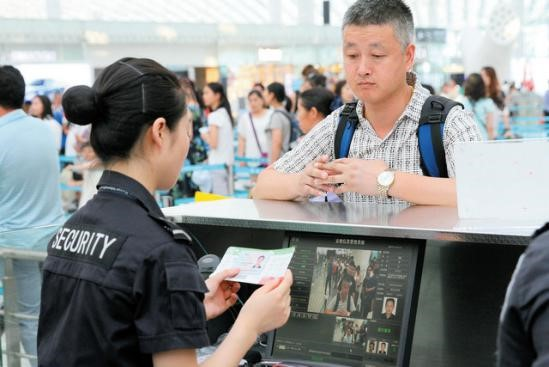
\includegraphics[height=4cm,width=0.4\textwidth]{fig//1-1-a.jpg} 
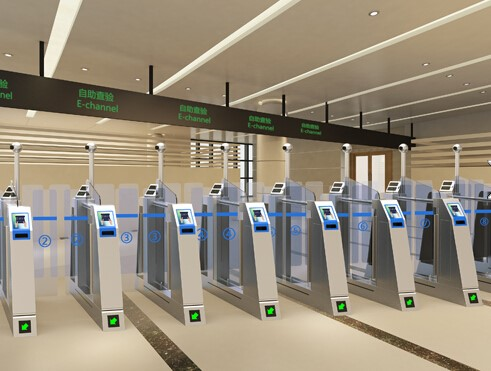
\includegraphics[height=4cm,width=0.4\textwidth]{fig//1-1-b.jpg} 
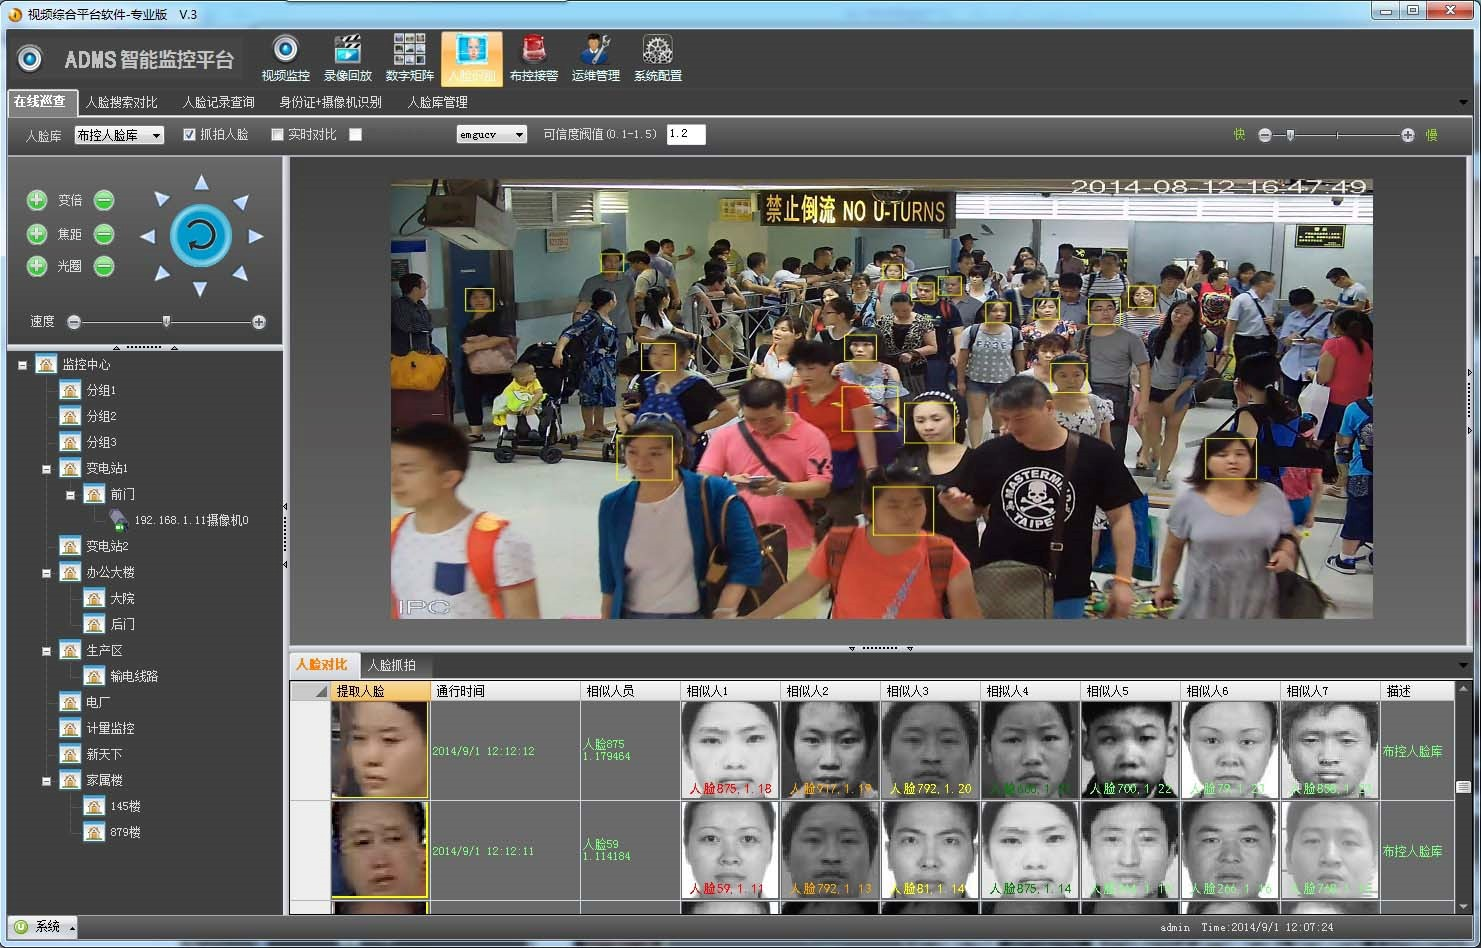
\includegraphics[height=4cm,width=0.4\textwidth]{fig//1-1-c.jpg} 
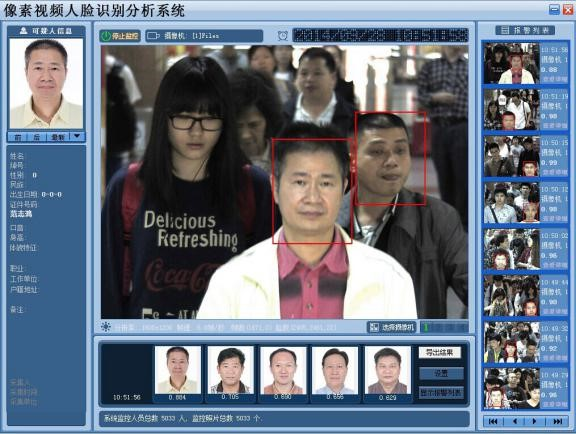
\includegraphics[height=4cm,width=0.4\textwidth]{fig//1-1-d.jpg}  
\fcaption{人脸分析与识别在安防自动化领域的应用}{The application of face analysis and recognition in the field of security automation.}    
\label{fig1:ND} 
\end{figure}

机器视觉技术的快速发展,提高了智能无人设备的普及率。人脸自动分析与识别是连接人和智能自动化系统重要接口之一。2017年,国务院参事、科学技术部原副部长刘燕华同志指出:“人与智能机器互动的时代正在到来,从人脸识别领域切入,平台机制将发挥巨大作用。智能机器不断向人类学习,会给人们的生活工作带来更多便利,使人的认知能力更加深入和精准,人可以借助智能技术对知识加工与整合”\cite{liu2013}。在安防领域很多情况都会用到人脸分析与识别技术,诸如国家出入境的检查、边境检查和刑事侦查等,进出公共场所的检查,还有汽车站、火车站和机场等人群密集的场所,课堂签到、寝室访问管理和中小学的安全接送等教育管理领域。随着科技不断发展,如图\ref{fig1:ND}和表\ref{tab1:facelingyu}所示,作为“智能设备”的连接入口,人脸分析与识别技术将有着巨大的应用前景。

\begin{table}[htbp]  %table 里面也可以嵌套tabular,只有tabular是不能加标题的
\linespread{0.5} 
\centering  %表格居中
\tcaption{人脸分析与识别的领域应用}{The applications of Face Analysis and Recognition} 
\label{tab1:facelingyu}
\begin{tabular}{lp{14cm}}  %右对齐
\midrule
领域&应用场景\\[1.5ex]
\hline
\multirow{4}{2cm}{安防领域}&门禁系统:\\&在楼宇、住宅小区、学校、工厂和企业等场所可以通过人脸识别辨识进入者身份。安全等级较高的地点也可使用人脸识别的门禁系统,未进行登记访问人员将触发警报系统。\\&摄像监视系统:\\&例如机场、银行、体育馆、商场、超级市场等公共场所,通过人脸识别装备对人群进行监视,进行身份识别和属性标定。同时疑犯的布控和追踪也是较为常见的公共安全应用场景。\\[2.5ex]

\multirow{6}{2cm}{商业领域}&广告精准投放:\\&人脸分析技术可快速准确的分析画面中出现的人物属性,如年龄、性别等信息,在广告投放方面可以给予一定的指导。\\&VIP客户管理:\\&通过人脸检索技术,可以识别图像中的人的身份,从而给予足够的关注和重视,提升用户体验。\\&人流监控:\\&通过人脸检测技术,可以轻松计算在画面里出现的人的数量,可以应用在零售行业分析货品摆放合理性,也可以应用在学校、公司、会议等场所进行统计。\\[2.5ex]

\multirow{4}{2cm}{娱乐领域}&相册分类:\\&通过人脸识别与人脸检索,可以聚合相册中的相似的人脸,轻松将照片按人脸进行智能分类。\\&美颜美妆:\\&五官定位技术可以精准定位五官的位置,实现人脸美颜美妆、人脸变形、人脸漫画、人脸换脸、人脸贴纸等。\\[2.5ex]

\bottomrule
\end{tabular}
\end{table}

人脸传达着非常丰富的信号,包括性别、年龄、表情和民族等等。人脸面部属性分析越来越受到各个研究领域的重视,如认知科学、心理学和神经科学等等。近年来由于机器视觉、人工智能技术、模式识别、图形学和机器学习等领域理论和技术的发展,人脸属性分析技术在各个领域发挥了巨大和广泛的影响力。由于国际交往和地区往来日益频繁,人脸属性的分析和比对在公共安全、边防安检都具有潜在的应用价值,如何隐式的、而非声明式的通过面部定量信息,推断人脸的相应属性信息是人脸自动化分析技术重要的分支之一。



\begin{table}[htbp]
\tcaption{不同$T$区域的人脸民族识别结果}{The results based on various ‘T’ regions}
\centering
\begin{tabular}{cccccccc}
\toprule
Region & $TP_{Rate}$ & $FP_{Rate}$ & $Precision$ & $Recall$ & $F-Measure$ & $Accuracy$ \\
\midrule
$O$ & 0.390	& 0.610	& 0.240	& 0.390	& 0.350	& 0.450\\
$T_1$ & 0.750 & 0.250 & 0.600 & 0.750 & 0.670 & 0.660\\
$T_2$ & 0.780 & 0.220 & 0.630 & 0.780 & 0.700 & 0.690\\
$T_3$ & 0.865 & 0.135 & 0.762 & 0.865 & 0.810 & 0.780\\
\bottomrule
\end{tabular}
\label{tb5:table_2}
\end{table}


\section{存在的主要问题}

通过上述论述可以看到,人脸民族特征提取、分析与识别在智能安防预警和人类学研究具有重要的科学意义和实际价值。但是在理论研究和算法技术上,还有很多问题需要进一步进行研究,还有很多难点需要克服。下面是本文在研究过程中总结的中国人脸民族特征研究中存在的问题。

\begin{enumerate}[(1)]


\item 问题一。

%\item 人脸民族分析的机器学习科学问题:人脸民族特征分析给传统机器学习方法带来了新问题,人脸的民族特征标注不仅对于数据集要求较大,同时对于标注也提出了新问题,因为人脸民族特征标注并不是简单的单标记学习问题,也不是完全的多标记学习问题,因此需要人脸民族特征识别和分析构建相应的识别方法和理论对问题进行定性。人脸民族特征分析也为相应的机器学习理论提供了有益的补充。

\item 问题二。
\item 问题二。

\item 如何利用构建有效的人脸民族特征方法。要准确、有效、快速识别和分析人脸的民族特征需要构建有效的算法对其进行分析,其中最重要的就是研究各种几何和图像特征对于人脸民族分析和识别的效果,在全局特征和局部特征中构建方法分析和识别人脸民族属性。

\item 小样本问题:中国多民族人脸库采集是较为困难的,需要保证样本民族信息准确性。如何通过技术手段扩大数据集规模也是研究过程中需要面对的问题之一。
\end{enumerate}


对测试样本筛选区分的方法,“全局表达方法”本文是指从全局考虑将所有训练样本的线性组合用测试样本的整体特征来表示,并通过各个类别的总训练样本和测试样本间的加权及差异的大小,据此对测试样本进行分类的方法,令$\boldsymbol{A} =  ( \boldsymbol{A}_1,\boldsymbol{A}_2,\cdots,\boldsymbol{A}_n )$表示原空间中的$n$个训练样本对应的向量。本文假定原空间中测试样本$y$可近似表达为所有训练样本的线性组合,即公式(\ref{eq5:11})所示。

\begin{equation}
\label{eq5:11}
y \approx \Sigma _{i=1}^n \boldsymbol{\beta}_i \boldsymbol{A}_i
\end{equation}

简便起见,本文将“近似等于”符号改写为“等于”。上式可改写为$ y = \boldsymbol{A\beta}$,式中$\boldsymbol{\beta}=(\boldsymbol{\beta}_1, \boldsymbol{\beta}_2,\cdots,\boldsymbol{\beta}_n )^T$,$\boldsymbol{A} =( \boldsymbol{A}_1,\boldsymbol{A}_2,\cdots,\boldsymbol{A}_n)$。

如果$\boldsymbol{A}^T \boldsymbol{A}$非奇异,则上式的最小平方误差解可依据 $\boldsymbol{beta}=(\boldsymbol{A}^T \boldsymbol{A})^{-1} \boldsymbol{A}^T y$求得。如果$\boldsymbol{A}^T\boldsymbol{A}$奇异,可依据 $\boldsymbol{\beta}=(\boldsymbol{A}^T \boldsymbol{A}+\gamma \boldsymbol{I})^{-1} \boldsymbol{A}^T y$求解,$\gamma $为正数,$\boldsymbol{I}$为单位矩阵。公式(\ref{eq5:11})表明每个训练样本均对测试样本的表达有贡献,其中第$i$个训练样本的贡献值为$\boldsymbol{\beta}_i \boldsymbol{A}_i$。假如来自第$k$类的所有训练样本为$\boldsymbol{A}_s,\cdots,\boldsymbol{A}_t$。则该类训练样本在表达测试样本上总贡献为:$g_k = \boldsymbol{\beta}_s \boldsymbol{A}_s+ \cdots +\boldsymbol{\beta}_t \boldsymbol{A}_t$. 其中$e_k = ||y -g_k ||^2$ 越小表示其属于第$k$类的贡献值越大。

\begin{equation}
\label{eq5:a}
\boldsymbol{A}=(\boldsymbol{X}^T \boldsymbol{X}+\mu \boldsymbol{I}) ^{-1} \boldsymbol{X}^T y
\end{equation}
式中:$I$表示单位矩阵

公式(\ref{f5:f5})中$ \boldsymbol{A}=[a_1,\cdots, a_K]^T$,数据样本$ \boldsymbol{X} =[x_1, \cdots , x_K]$要求$XA$ 与测试样本$y$之间偏差最小,且解向量$\boldsymbol{A}$的范数较小,将下式函数最小化作为目标函数,公式(\ref{eq5:la})所示。

\begin{equation}
\label{eq5:la}
L(\boldsymbol{A})=||y-\boldsymbol{XA}||^2 + \mu ||\boldsymbol{A}||^2 =(y-\boldsymbol{XA})^T(y-\boldsymbol{XA})+ \mu \boldsymbol{A}^T\boldsymbol{A}
\end{equation}
公式(\ref{eq5:la})为正常数,$\mu$ 表示一正的常数。依据拉格朗日方法,最优的$\boldsymbol{A}$应满足${\frac {\partial L(\boldsymbol{A})}{\partial \boldsymbol{A}}} = 0$。 因此,快速稀疏描述方法的最优解,如公式(\ref{eq5:la})所示。

\section{本文的主要工作}

第一章主要介绍了本课题的研究背景和重要意义,以及研究的方向、研究内容和主要工作,说明本课题的可行性。

第二章介绍人脸检测方法,实现对人脸的眼部和嘴部特征点定位。

第三章介绍基于眼部的疲劳检测方法,获得实验结果并对结果进行分析,结合实际情况,优化基于眼部的疲劳检测方法,获得根据眼部特征判断疲劳的阈值,证明疲劳检测方法的可能性存在。

第四章介绍基于嘴部打哈欠的疲劳检测方法,获得实验结果并对结果进行分析。

第五章概述基于ARM处理器开发基于人脸识别的疲劳检测系统,并介绍测试环境所需的开发环境与工具库,包括:ARM处理器、Android Studio等,结合实际情况,将眼部疲劳检测方法和嘴部打哈欠状态相结合,证明结合后新的疲劳检测方法的可能性存在,将其嵌入在移动系统中,并对该系统做了相关的性能分析与实验测试,得出实验结论。
第六章总结全文的工作,并对下一步工作进行展望。






























%\include{data/chap02}
%\include{data/chap04}
%\include{data/chap03}
%\include{data/chap05}
%\include{data/chap06}
%\include{data/chap07}
%%% 其它部分
\backmatter

% 本科生要这几个索引,研究生不要。选择性留下。
\makeatletter
\ifthu@bachelor
  % 插图索引
  \listoffigures
  % 表格索引
  \listoftables
  % 公式索引
  \listofequations
\fi
\makeatother


% 参考文献
\bibliographystyle{style/thubib_2}
%\bibliographystyle{zjugbno}
\bibliography{ref/refs}


%% 致谢

%%% Local Variables:
%%% mode: latex
%%% TeX-master: "../main"
%%% End:

\begin{ack}
   (致谢要自己好好写,会被查重的,要重视)
 岁月如歌,光阴似箭,两年的研究生生活即将结束。经历了找工作的喧嚣与坎坷,我深深体会到了写作论文时的那份宁静与思考。回首两年的求学历程,对那些引导我、帮助我、激励我的人,我心中充满了感激。

   首先要感谢导师XX教授,论文定题到写作定稿,倾注了许老师大量的心血。在我攻读硕士研究生期间,深深受益于许老师的关心、爱护和谆谆教导。他作为老师,点拨迷津,让人如沐春风;作为长辈,关怀备至,让人感念至深。能师XXXXXX老师,我为自己感到庆幸。在此谨向XXX老师表示我最诚挚的敬意和感谢!

   还要感谢XXX教授。李老师在论文的写作中给予了许多指导与建议,谨在此表示衷心的感谢。

   同时,我要感谢所有教导过我、关心过我的老师。特别是统计学院的XXX教授XX老师。你们为我的学业倾注了大量心血,你们为人师表的风范令我敬仰,严谨治学的态度令我敬佩。还要感谢感谢XX老师其他各位老师对我的一贯帮助!

   感谢一直关心与支持我的同学和朋友们!我的朋友,XXX,感谢你们的鼓励和帮助。还要感谢的是我寝室的姐妹XXX,师兄XXX以及统计学院2005级全体研究生同学。两年来,我们朝夕相处,共同进步,感谢你们给予我的所有关心和帮助。同窗之谊,我将终生难忘!

   在此要感谢我生活学习了六年的母校——湖南大学,母校给了我一个宽阔的学习平台,让我不断吸取新知,充实自己。

   需要特别感谢的是我的父母。父母的养育之恩无以为报,他们是我十多年求学路上的坚强后盾,在我面临人生选择的迷茫之际,为我排忧解难,他们对我无私的爱与照顾是我不断前进的动力。
\end{ack}


% 附录
\begin{appendix}
%%%% Local Variables: 
%%% mode: latex
%%% TeX-master: "../main"
%%% End: 

\chapter{外文资料原文}
\label{cha:engorg}
As one of the most widely used techniques in operations research, {\em
  mathematical programming} is defined as a means of maximizing a quantity known
as {\em objective function}, subject to a set of constraints represented by
equations and inequalities. Some known subtopics of mathematical programming are
linear programming, nonlinear programming, multiobjective programming, goal
programming, dynamic programming, and multilevel programming$^{[1]}$.

It is impossible to cover in a single chapter every concept of mathematical
programming. This chapter introduces only the basic concepts and techniques of
mathematical programming such that readers gain an understanding of them
throughout the book$^{[2,3]}$.


\section{Single-Objective Programming}
The general form of single-objective programming (SOP) is written
as follows,
\begin{equation}\tag*{(123)} % 如果附录中的公式不想让它出现在公式索引中,那就请
                             % 用 \tag*{xxxx}
\left\{\begin{array}{l}
\max \,\,f(x)\\[0.1 cm]
\mbox{subject to:} \\ [0.1 cm]
\qquad g_j(x)\le 0,\quad j=1,2,\cdots,p
\end{array}\right.
\end{equation}
which maximizes a real-valued function $f$ of
$x=(x_1,x_2,\cdots,x_n)$ subject to a set of constraints.

\newtheorem{mpdef}{Definition}[chapter]
\begin{mpdef}
In SOP, we call $x$ a decision vector, and
$x_1,x_2,\cdots,x_n$ decision variables. The function
$f$ is called the objective function. The set
\begin{equation}\tag*{(456)} % 这里同理,其它不再一一指定。
S=\left\{x\in\Re^n\bigm|g_j(x)\le 0,\,j=1,2,\cdots,p\right\}
\end{equation}
is called the feasible set. An element $x$ in $S$ is called a
feasible solution.
\end{mpdef}

\newtheorem{mpdefop}[mpdef]{Definition}
\begin{mpdefop}
A feasible solution $x^*$ is called the optimal
solution of SOP if and only if
\begin{equation}
f(x^*)\ge f(x)
\end{equation}
for any feasible solution $x$.
\end{mpdefop}

One of the outstanding contributions to mathematical programming was known as
the Kuhn-Tucker conditions\ref{eq:ktc}. In order to introduce them, let us give
some definitions. An inequality constraint $g_j(x)\le 0$ is said to be active at
a point $x^*$ if $g_j(x^*)=0$. A point $x^*$ satisfying $g_j(x^*)\le 0$ is said
to be regular if the gradient vectors $\nabla g_j(x)$ of all active constraints
are linearly independent.

Let $x^*$ be a regular point of the constraints of SOP and assume that all the
functions $f(x)$ and $g_j(x),j=1,2,\cdots,p$ are differentiable. If $x^*$ is a
local optimal solution, then there exist Lagrange multipliers
$\lambda_j,j=1,2,\cdots,p$ such that the following Kuhn-Tucker conditions hold,
\begin{equation}
\label{eq:ktc}
\left\{\begin{array}{l}
    \nabla f(x^*)-\sum\limits_{j=1}^p\lambda_j\nabla g_j(x^*)=0\\[0.3cm]
    \lambda_jg_j(x^*)=0,\quad j=1,2,\cdots,p\\[0.2cm]
    \lambda_j\ge 0,\quad j=1,2,\cdots,p.
\end{array}\right.
\end{equation}
If all the functions $f(x)$ and $g_j(x),j=1,2,\cdots,p$ are convex and
differentiable, and the point $x^*$ satisfies the Kuhn-Tucker conditions
(\ref{eq:ktc}), then it has been proved that the point $x^*$ is a global optimal
solution of SOP.

\subsection{Linear Programming} 
\label{sec:lp}

If the functions $f(x),g_j(x),j=1,2,\cdots,p$ are all linear, then SOP is called
a {\em linear programming}.

The feasible set of linear is always convex. A point $x$ is called an extreme
point of convex set $S$ if $x\in S$ and $x$ cannot be expressed as a convex
combination of two points in $S$. It has been shown that the optimal solution to
linear programming corresponds to an extreme point of its feasible set provided
that the feasible set $S$ is bounded. This fact is the basis of the {\em simplex
  algorithm} which was developed by Dantzig as a very efficient method for
solving linear programming.
\begin{table}[ht]
\centering
  \centering
  \caption*{Table~1\hskip1em This is an example for manually numbered table, which
    would not appear in the list of tables}
  \label{tab:badtabular2}
  \begin{tabular}[c]{|c|m{0.8in}|c|c|c|c|c|}\hline
    \multicolumn{2}{|c|}{Network Topology} & \# of nodes & 
    \multicolumn{3}{c|}{\# of clients} & Server \\\hline
    GT-ITM & Waxman Transit-Stub & 600 &
    \multirow{2}{2em}{2\%}& 
    \multirow{2}{2em}{10\%}& 
    \multirow{2}{2em}{50\%}& 
    \multirow{2}{1.2in}{Max. Connectivity}\\\cline{1-3}
    \multicolumn{2}{|c|}{Inet-2.1} & 6000 & & & &\\\hline
    \multirow{2}{1in}{Xue} & Rui  & Ni &\multicolumn{4}{c|}{\multirow{2}*{\thuthesis}}\\\cline{2-3}
    & \multicolumn{2}{c|}{ABCDEF} &\multicolumn{4}{c|}{} \\\hline
\end{tabular}  
\end{table}

Roughly speaking, the simplex algorithm examines only the extreme points of the
feasible set, rather than all feasible points. At first, the simplex algorithm
selects an extreme point as the initial point. The successive extreme point is
selected so as to improve the objective function value. The procedure is
repeated until no improvement in objective function value can be made. The last
extreme point is the optimal solution.

\subsection{Nonlinear Programming}

If at least one of the functions $f(x),g_j(x),j=1,2,\cdots,p$ is nonlinear, then
SOP is called a {\em nonlinear programming}.

A large number of classical optimization methods have been developed to treat
special-structural nonlinear programming based on the mathematical theory
concerned with analyzing the structure of problems.
\begin{figure}[h]
  \centering
  \includegraphics[clip]{thu-lib-logo}
  \caption*{Figure~1\hskip1em This is an example for manually numbered figure,
    which would not appear in the list of figures}
  \label{tab:badfigure2}    
\end{figure}

Now we consider a nonlinear programming which is confronted solely with
maximizing a real-valued function with domain $\Re^n$.  Whether derivatives are
available or not, the usual strategy is first to select a point in $\Re^n$ which
is thought to be the most likely place where the maximum exists. If there is no
information available on which to base such a selection, a point is chosen at
random. From this first point an attempt is made to construct a sequence of
points, each of which yields an improved objective function value over its
predecessor. The next point to be added to the sequence is chosen by analyzing
the behavior of the function at the previous points. This construction continues
until some termination criterion is met. Methods based upon this strategy are
called {\em ascent methods}, which can be classified as {\em direct methods},
{\em gradient methods}, and {\em Hessian methods} according to the information
about the behavior of objective function $f$. Direct methods require only that
the function can be evaluated at each point. Gradient methods require the
evaluation of first derivatives of $f$. Hessian methods require the evaluation
of second derivatives. In fact, there is no superior method for all
problems. The efficiency of a method is very much dependent upon the objective
function.

\subsection{Integer Programming}

{\em Integer programming} is a special mathematical programming in which all of
the variables are assumed to be only integer values. When there are not only
integer variables but also conventional continuous variables, we call it {\em
  mixed integer programming}. If all the variables are assumed either 0 or 1,
then the problem is termed a {\em zero-one programming}. Although integer
programming can be solved by an {\em exhaustive enumeration} theoretically, it
is impractical to solve realistically sized integer programming problems. The
most successful algorithm so far found to solve integer programming is called
the {\em branch-and-bound enumeration} developed by Balas (1965) and Dakin
(1965). The other technique to integer programming is the {\em cutting plane
  method} developed by Gomory (1959).

\hfill\textit{Uncertain Programming\/}\quad(\textsl{BaoDing Liu, 2006.2})

\section*{References}
\noindent{\itshape NOTE: these references are only for demonstration, they are
  not real citations in the original text.}

\begin{enumerate}[{$[$}1{$]$}]
\item Donald E. Knuth. The \TeX book. Addison-Wesley, 1984. ISBN: 0-201-13448-9
\item Paul W. Abrahams, Karl Berry and Kathryn A. Hargreaves. \TeX\ for the
  Impatient. Addison-Wesley, 1990. ISBN: 0-201-51375-7
\item David Salomon. The advanced \TeX book.  New York : Springer, 1995. ISBN:0-387-94556-3
\end{enumerate}

\chapter{外文资料的调研阅读报告或书面翻译}
\section{单目标规划}
北冥有鱼,其名为鲲。鲲之大,不知其几千里也。化而为鸟,其名为鹏。鹏之背,不知其几
千里也。怒而飞,其翼若垂天之云。是鸟也,海运则将徙于南冥。南冥者,天池也。 
\begin{equation}\tag*{(123)}
 p(y|\mathbf{x}) = \frac{p(\mathbf{x},y)}{p(\mathbf{x})}=
\frac{p(\mathbf{x}|y)p(y)}{p(\mathbf{x})}
\end{equation}

吾生也有涯,而知也无涯。以有涯随无涯,殆已!已而为知者,殆而已矣!为善无近名,为
恶无近刑,缘督以为经,可以保身,可以全生,可以养亲,可以尽年。

\subsection{线性规划}
庖丁为文惠君解牛,手之所触,肩之所倚,足之所履,膝之所倚,砉然响然,奏刀騞然,莫
不中音,合于桑林之舞,乃中经首之会。
\begin{table}[ht]
\centering
  \centering
  \caption*{表~1\hskip1em 这是手动编号但不出现在索引中的一个表格例子}
  \label{tab:badtabular3}
  \begin{tabular}[c]{|c|m{0.8in}|c|c|c|c|c|}\hline
    \multicolumn{2}{|c|}{Network Topology} & \# of nodes & 
    \multicolumn{3}{c|}{\# of clients} & Server \\\hline
    GT-ITM & Waxman Transit-Stub & 600 &
    \multirow{2}{2em}{2\%}& 
    \multirow{2}{2em}{10\%}& 
    \multirow{2}{2em}{50\%}& 
    \multirow{2}{1.2in}{Max. Connectivity}\\\cline{1-3}
    \multicolumn{2}{|c|}{Inet-2.1} & 6000 & & & &\\\hline
    \multirow{2}{1in}{Xue} & Rui  & Ni &\multicolumn{4}{c|}{\multirow{2}*{\thuthesis}}\\\cline{2-3}
    & \multicolumn{2}{c|}{ABCDEF} &\multicolumn{4}{c|}{} \\\hline
\end{tabular}  
\end{table}

文惠君曰:“嘻,善哉!技盖至此乎?”庖丁释刀对曰:“臣之所好者道也,进乎技矣。始臣之
解牛之时,所见无非全牛者;三年之后,未尝见全牛也;方今之时,臣以神遇而不以目视,
官知止而神欲行。依乎天理,批大郤,导大窾,因其固然。技经肯綮之未尝,而况大坬乎!
良庖岁更刀,割也;族庖月更刀,折也;今臣之刀十九年矣,所解数千牛矣,而刀刃若新发
于硎。彼节者有间而刀刃者无厚,以无厚入有间,恢恢乎其于游刃必有余地矣。是以十九年
而刀刃若新发于硎。虽然,每至于族,吾见其难为,怵然为戒,视为止,行为迟,动刀甚微,
謋然已解,如土委地。提刀而立,为之而四顾,为之踌躇满志,善刀而藏之。”

文惠君曰:“善哉!吾闻庖丁之言,得养生焉。”


\subsection{非线性规划}
孔子与柳下季为友,柳下季之弟名曰盗跖。盗跖从卒九千人,横行天下,侵暴诸侯。穴室枢
户,驱人牛马,取人妇女。贪得忘亲,不顾父母兄弟,不祭先祖。所过之邑,大国守城,小
国入保,万民苦之。孔子谓柳下季曰:“夫为人父者,必能诏其子;为人兄者,必能教其弟。
若父不能诏其子,兄不能教其弟,则无贵父子兄弟之亲矣。今先生,世之才士也,弟为盗
跖,为天下害,而弗能教也,丘窃为先生羞之。丘请为先生往说之。”
\begin{figure}[h]
  \centering
  \includegraphics{hello}
  \caption*{图~1\hskip1em 这是手动编号但不出现索引中的图片的例子}
  \label{tab:badfigure3}    
\end{figure}

柳下季曰:“先生言为人父者必能诏其子,为人兄者必能教其弟,若子不听父之诏,弟不受
兄之教,虽今先生之辩,将奈之何哉?且跖之为人也,心如涌泉,意如飘风,强足以距敌,
辩足以饰非。顺其心则喜,逆其心则怒,易辱人以言。先生必无往。”

孔子不听,颜回为驭,子贡为右,往见盗跖。

\subsection{整数规划}
盗跖乃方休卒徒大山之阳,脍人肝而餔之。孔子下车而前,见谒者曰:“鲁人孔丘,闻将军
高义,敬再拜谒者。”谒者入通。盗跖闻之大怒,目如明星,发上指冠,曰:“此夫鲁国之
巧伪人孔丘非邪?为我告之:尔作言造语,妄称文、武,冠枝木之冠,带死牛之胁,多辞缪
说,不耕而食,不织而衣,摇唇鼓舌,擅生是非,以迷天下之主,使天下学士不反其本,妄
作孝弟,而侥幸于封侯富贵者也。子之罪大极重,疾走归!不然,我将以子肝益昼餔之膳。”


\chapter{其它附录}
前面两个附录主要是给本科生做例子。其它附录的内容可以放到这里,当然如果你愿意,可
以把这部分也放到独立的文件中,然后将其 \verb|\input| 到主文件中。
\end{appendix}

% 个人简历
%%最终用
\documentclass{standalone}
% preamble: usepackage, etc.
\begin{document}    
\thesisresume


%个人简历居中显示
%\begin{center} 
%	\heiti \sihao 个人简历
%\end{center}

    
\section*{个人简历}
\noindent 姓名:xxx\\
性别:xx\
出生年月:xxxx年xx月x日\\
籍贯:xxxxxx\\
研究方向:xxxxxx\\
教育经历:\\
xxx\\
xxx

\section*{攻读硕士学位期间取得的科研成果} % 发表的和录用的合在一起
\begin{enumerate}
\renewcommand{\labelenumi}{[\theenumi]}
\item 
T. G. Dietterich, R. H. Lathrop and T. Lozano-Pérez. Solving the multiple-instance problem with axis-parallel rectangles. Artificial Intelligence, 1997, 89(1-2): 31-71.
\end{enumerate}

\section*{攻读硕士学位期间主持或参加的科研项目}
\begin{enumerate}
\renewcommand{\labelenumi}{[\theenumi]}
\item 国家自然科学基金面上项目(6xxx2):xxx在xxx及其应用,2016.1—2020.12,负责人:
xxx。  
\end{enumerate}

\end{document}
%盲审用
%\begin{resume}

  \resumeitem{个人简历}

%  1980年2月3日出生于吉林省辽源市;
%
%  2002年5月考入东北大学计算机软件与理论专业,2005 年5月获得工学硕士学位;
%  
%  2005年6月至今,大连民族大学计算机科学与工程学院,教师;
%  
%  2010年9月考入东北大学控制理论与控制工程专业在职攻读博士学位。


  \resumeitem{第一作者发表/录用的学术论文} % 发表的和录用的合在一起

  \begin{enumerate}[{[}1{]}]  

\item 第一作者. Facial semantic representation for ethnical Chinese minorities based on geometric similarity[J]. International Journal of Machine Learning \& Cybernetics, 2017(Pt 3):1-21.(SCI刊源,在线发表)
  
%\item WANG Cun-Rui, ZHANG Qing-Ling, DUAN Xiao-Dong, WANG Yuan-Gang, LI Ze-Dong. Research of Face Ethnic Features from Manifold Structure. Acta Automatica Sinica, 2018, 44(1): 140-159.
  
\item 第一作者. Multi-ethnical Chinese Facial Characterization and Analysis   Multimedia Tools and Applications.  (DOI: 10.1007/s11042-018-6018-1)(SCI刊源,已录用)

\item 第一作者. Facial Feature Discovery for Ethnicity Recognition[J]. WIREs Data Mining and Knowledge Discovery (DMKD-00355) (SCI刊源,已录用)

\item 第一作者.  基于流形结构的人脸民族特征研究[J]. 自动化学报, 2018, 44(1). (EI检索期刊,已刊发)

\item 第一作者.  基于尺度聚类仿射过滤的图像拼接算法[J]. 东北大学学报(自然科学版), 2011, 32(7):917-921. EI检索期刊,已刊发)

%\item 第一作者.   A network weight-based Multi-Community discovery Algorithm[C]. Third International Workshop on Advanced Computational Intelligence. IEEE, 2010:570 - 574.


\item 第一作者. 生物地理学优化算法综述[J]. 计算机科学, 2010, 37(7):34-38.
%\item 第一作者. 一种基于SIFT的网格仿射拼接算法[J]. 计算机工程与应用, 2011, 47(36):187-189.
    

\end{enumerate}
\resumeitem{合作发表的学术论文}
\begin{enumerate}[{[}1{]}]
\item  第四作者. Multi-ethnic facial features extraction based on axiomatic fuzzy set theory[J], Neurocomputing, 2017, 242, 161-177. (SCI检索号:000399859500014)

\item 第四作者. New semantic descriptor construction for facial expression[J], Multimedia Tools and Applications,DOI: 10.1007/s11042-017-4818-3.(SCI, 已录用)

\item 第三作者. 基于AFS的多民族人脸语义描述与挖掘方法研究[J]. 计算机学报, 2016, 39(7):1435-1449.

\item 第五作者. AFSNN: a classification algorithm using axiomatic fuzzy sets and neural networks[J]. \textbf{IEEE Transactions on Fuzzy Systems}, 2018, 10.1109/TFUZZ.2017.2788875.\textbf{(SCI,已发表})

\item 第四作者. A spectral clustering method with semantic description based on axiomatic fuzzy sets theory[J]. \textbf{Applied Soft Computing}, 2018, 64:59-74. \textbf{(SCI, 已发表)}

%\item Yuangang Wang, Xiaodong Duan, Xiaodong Liu, Cunrui Wang, Zedong Li. Semantic description method for face features of larger Chinese ethnic groups based on improved WM method[J]. \textbf{Neurocomputing}, 2016, 175: 515-528. \textbf{(SCI,已发表)}

\item 第三作者.  Comparison and Fusion of Multiple Types of Features for Image-Based Facial Beauty Prediction[C]. Chinese Conference on Biometric Recognition. Springer, Cham, 2017:23-30.

\item 第四作者.  Semantic description method for face features of larger Chinese ethnic groups based on improved WM method[J]. Neurocomputing, 2016, 175(PA):515-528.

\item 第四作者.  A Computational Other-Race-Effect Analysis for 3D Facial Expression Recognition[M]. Biometric Recognition. Springer International Publishing, 2016:483-493.

\item 第三作者. Research on Facial Features of Major Chinese Nationalities[J]. Applied Mechanics \& Materials, 2014, 687-691:837-840.


	\end{enumerate}

\resumeitem{研究成果} % 有就写,没有就删除
  \begin{enumerate}[{[}1{]}]
  \item 人脸信息采集系统: 中国,2013SR008567. (软件著作权.)
  \item 人脸2D-3D模型构建系统: 中国,2013SR008932. (软件著作权.)
  \end{enumerate}
  
  
  {\large 参加的科研项目}
\begin{enumerate}
\item 国家自然科学基金项目“基于族群谱系特征的多民族表情理解研”(61370146),主要参与者。

\item 国家自然科学基金项目``眼睛与面部动作在自发表情中的协同机制研究及应用”(61672132)“,主要参与者。
\end{enumerate}

\newpage
\quad

\end{resume}

\end{document}